%%This is a very basic article template.
%%There is just one section and two subsections.
\documentclass{article}
\usepackage[latin1]{inputenc} %coding of writteninput %latin1 allows for Umlaute
\usepackage[T1]{fontenc}%vectorized fonts (cm-super package)
\usepackage[german]{babel}%some specifics of the german language
\usepackage{amsfonts, amsmath, amsthm, amssymb, paralist} 
  \usepackage{listings}
\usepackage{geometry}
  \geometry{a4paper, top=25mm, left=20mm, right=15mm, bottom=20mm, headsep=10mm, footskip=12mm}
 \usepackage{rotating} 
 %Decisiontree
 \usepackage{tikz,forest}
\usetikzlibrary{arrows.meta}
  
\usepackage{graphicx} 

\usepackage{verbatim}%f�r txt datei

\usepackage{color} %red, green, blue, yellow, cyan, magenta, black, white
\definecolor{mygreen}{RGB}{28,172,0} % color values Red, Green, Blue
\definecolor{mylilas}{RGB}{170,55,241}
\usepackage{pdfpages}
\usepackage[section]{placeins}

\title{Assignment 1}

\begin{document}
 \setlength{\parindent}{0em}

\section*{Exerise 1}
\subsection*{a)}
The VC-dimension is 3, because you can shatter all sets of size 3, but it is not
possible to shatter the set $\{+-+-\}$. Like to see in the following picture:

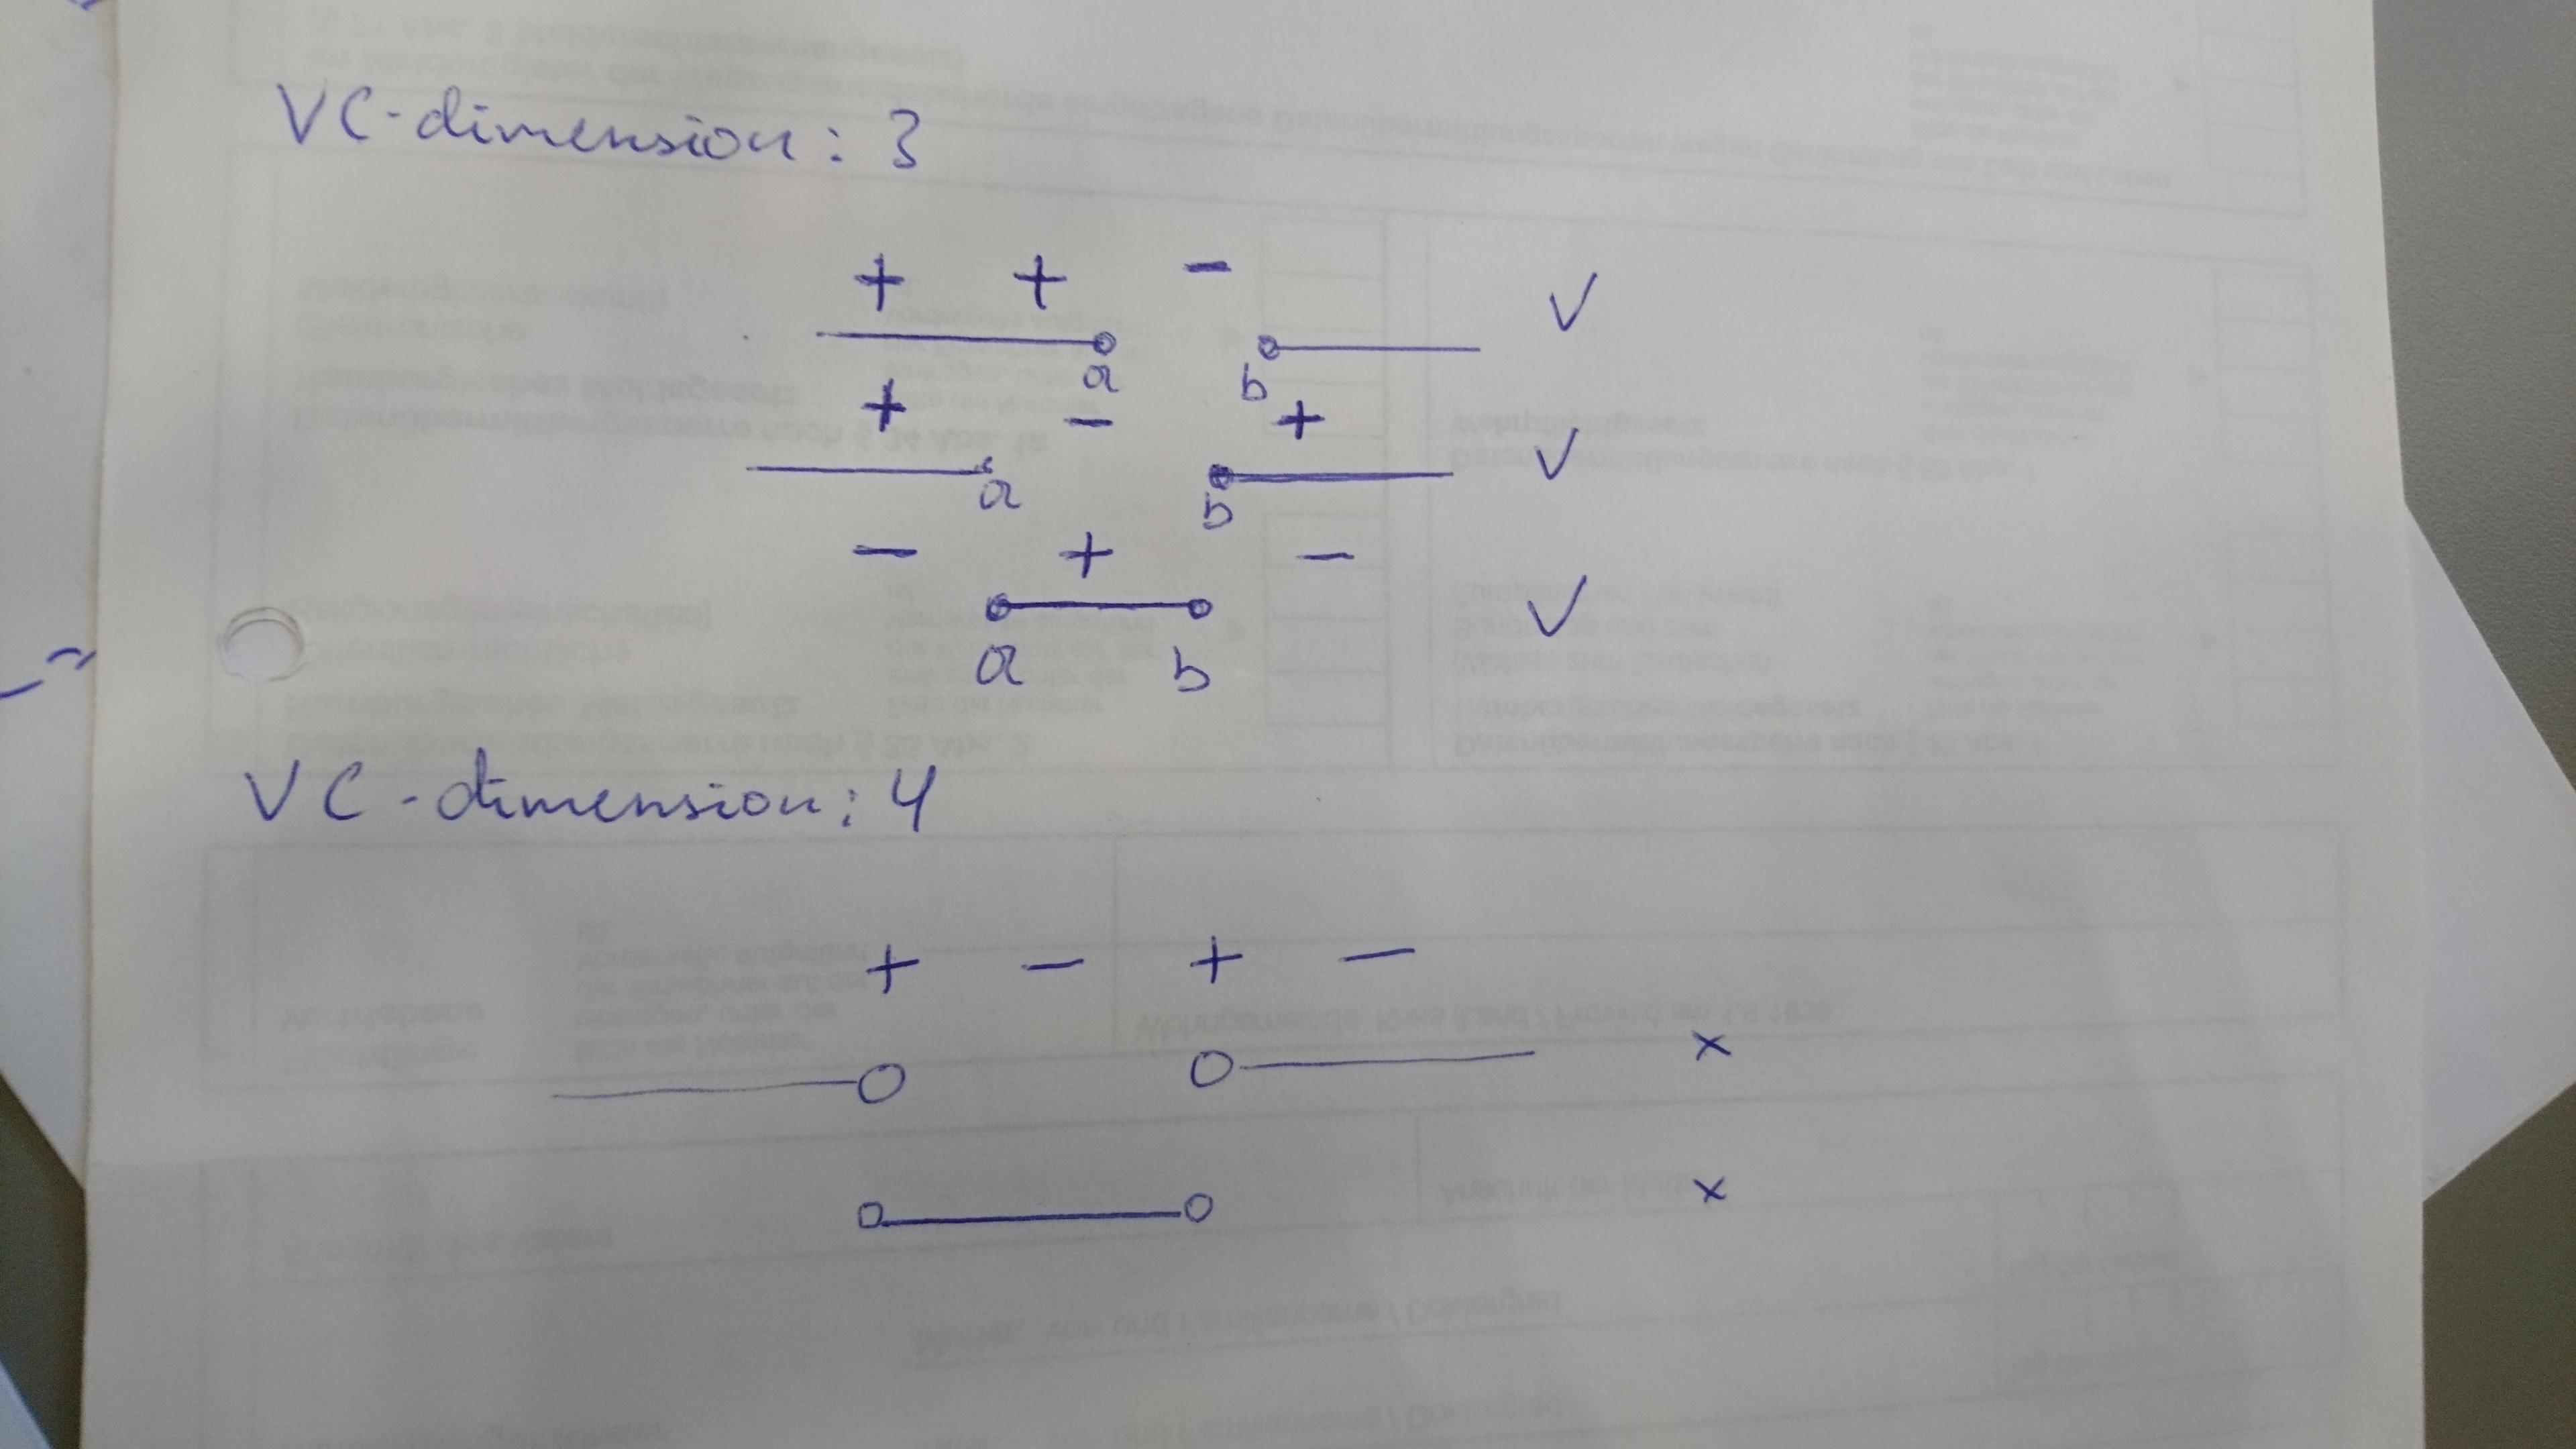
\includegraphics[width=.6\linewidth]{1a.jpg}

\subsection*{b)}

The VC-dimension is $\infty$, 

You construct the set as following:
\begin{enumerate}
  \item Use only primenumbers as basis for construction $B=\{p_1,\ldots,p_k\}$
  \item As set $X$, you want to shatter, use the product of the numbers in
  $B/p_i$ for a $p_i$
  \item The $p_i$, that you doesn't used, is the greatest common divisor of the
  other numbers
  \item If you want to shatter such a set, than the primenumbers you do not have
  in the products are the $k$ you need to use.
  \item This construction is possible for $\infty$ many combinations
\end{enumerate}
\begin{tabular}{|c|c|c|c|c|}
	  &$p_1$ &$p_2$ &$p_3$ &$p_4$\\
$x_1$ &		 &1		&1	   &1\\
$x_2$ &1	 &		&1	   &1\\
$x_3$ &1	 &1		&	   &1\\
$x_4$ &1	 &1		&1	   & \\
\end{tabular}
\section*{Exercise 2}
The first observation is, the points have to be in a circle. Wouldn't they be in
a circle, there would always be a point in the middle or a little bit outside, that destroys the ability of shattering. The points outside and the point in the middle would have to be of
the same ``classification''. Also is the class of the point a little bit outside directly defined, because of the points closer to the rest.

It is possible to sort 7 points such that they can be shattered by arbitrary rectangles in the plane. Capturing of subsets of size 1
and 2 are trivial. In the pictures below, you can see the examples how subsets of 4 and 3 points can be captured. The circle
is symmetric, so you can turn the picture in all directions and it will still work out.

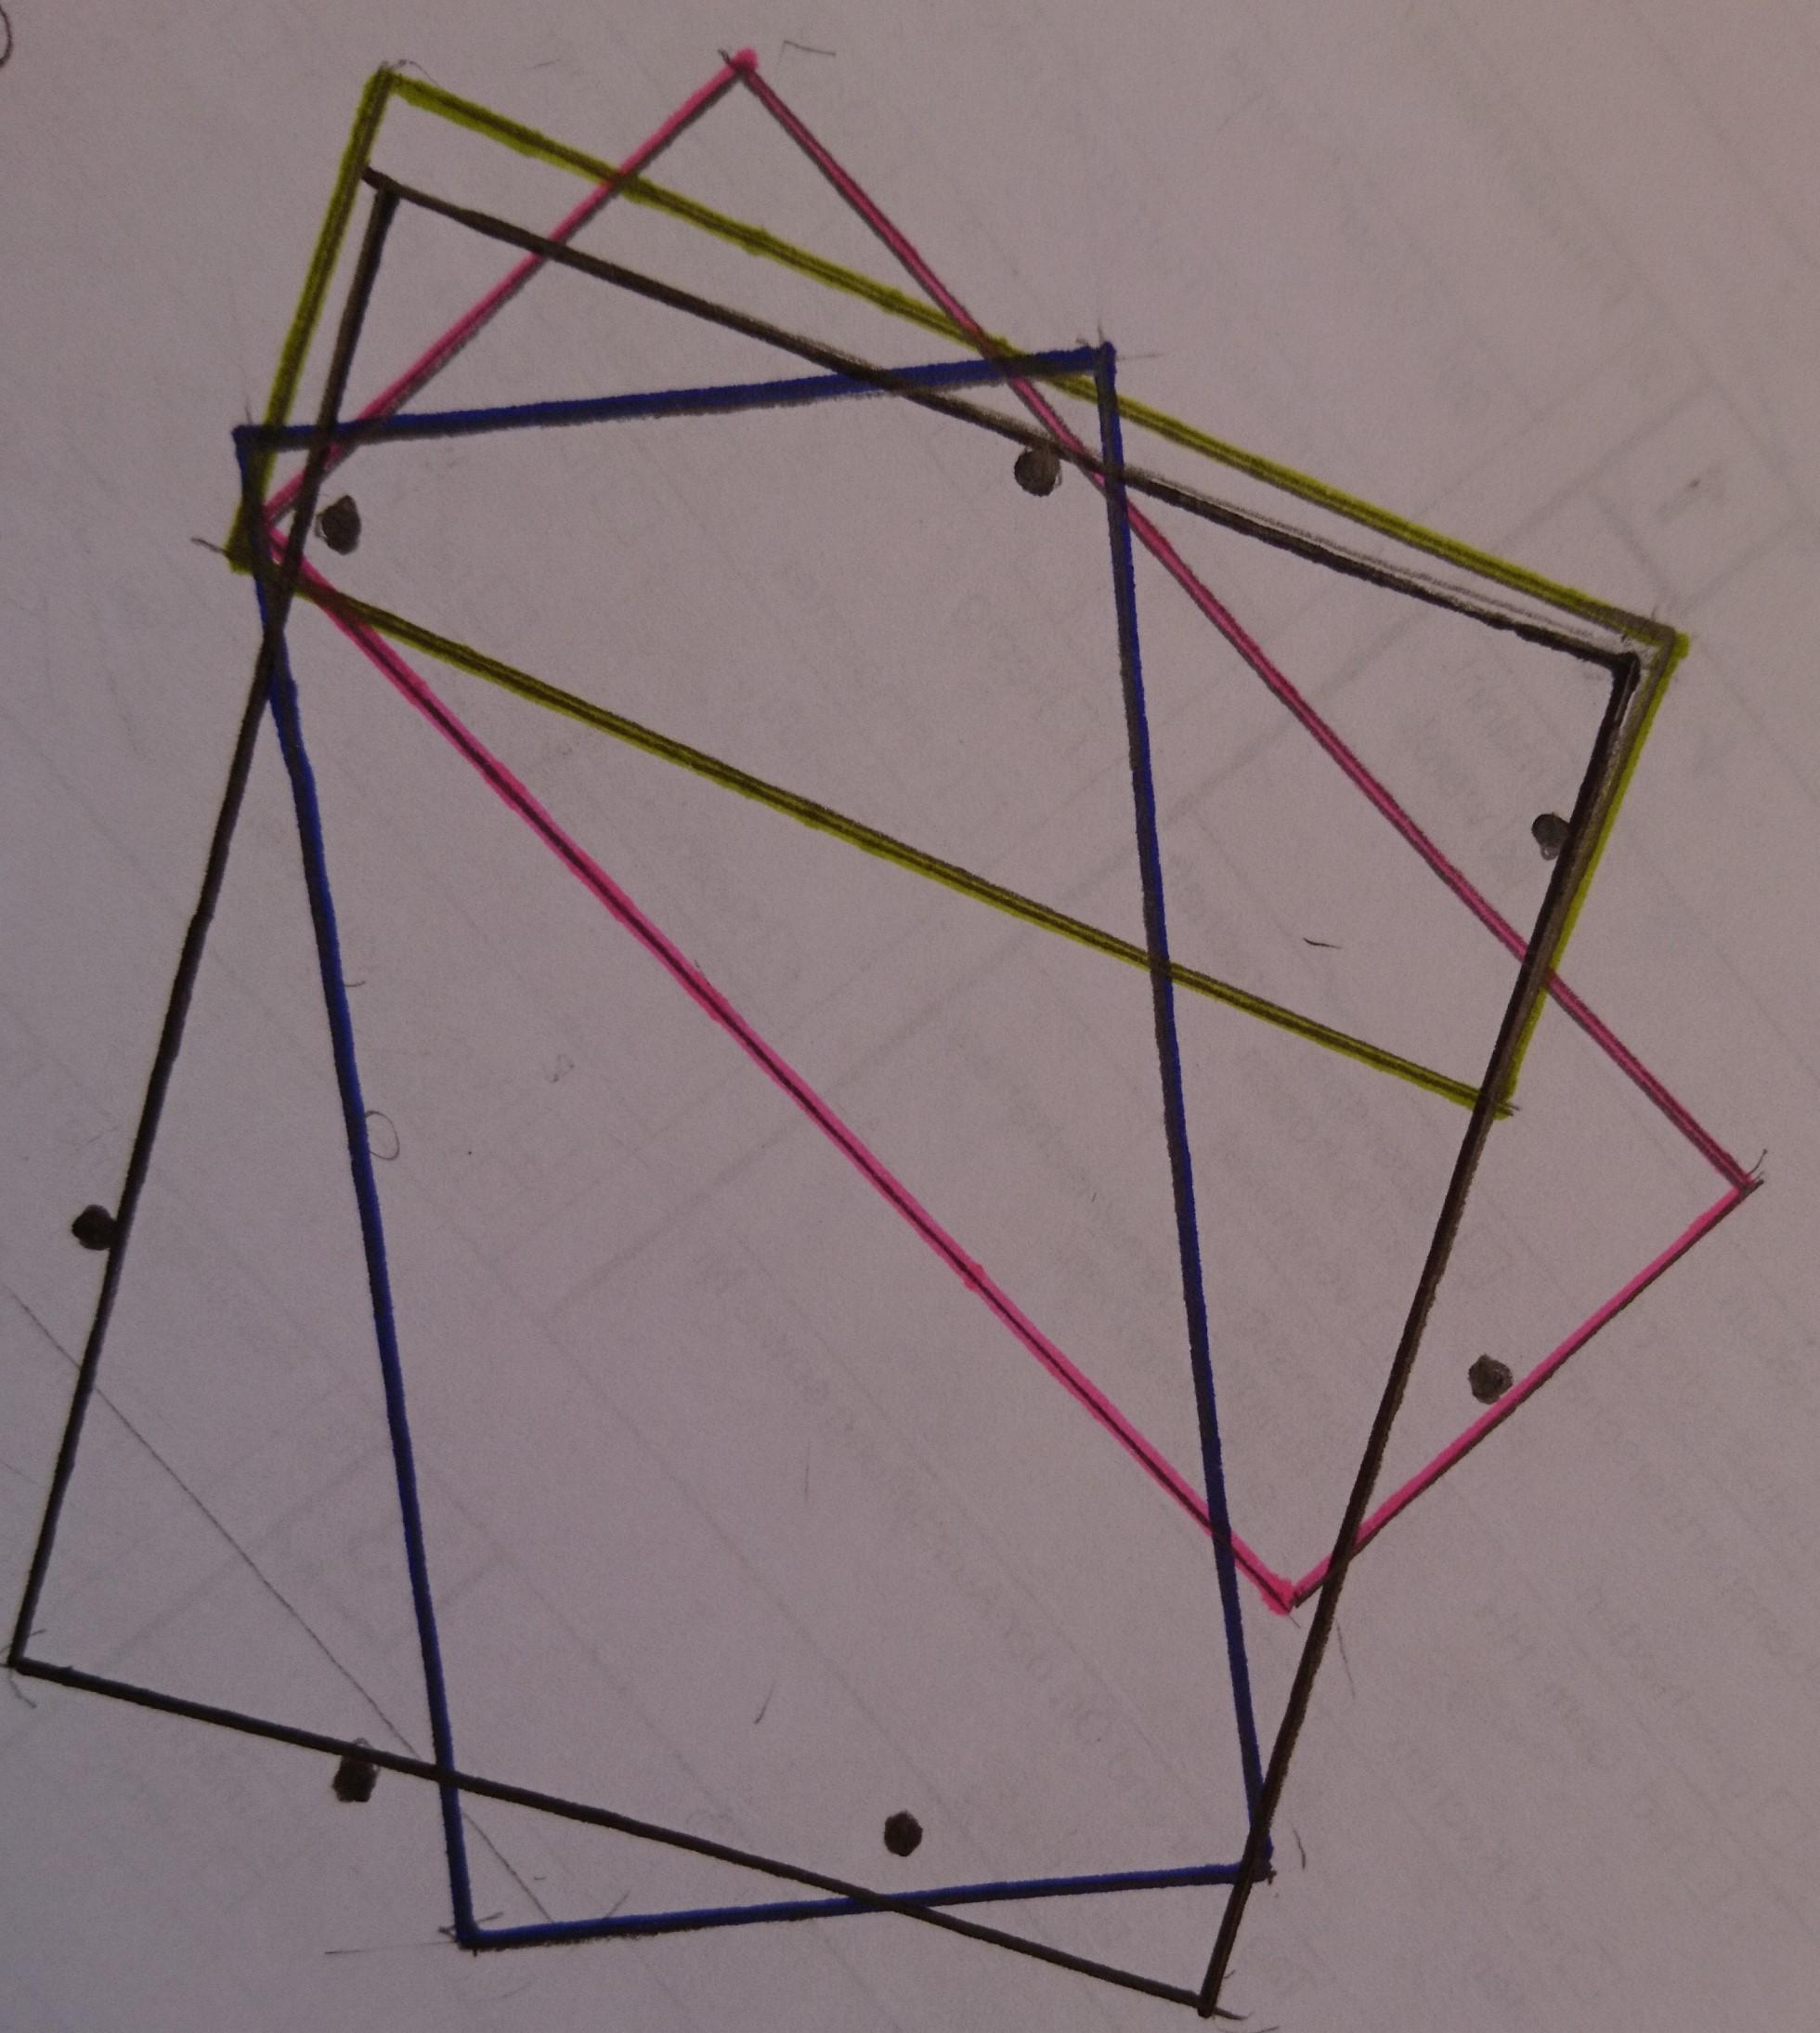
\includegraphics[width=.6\linewidth]{2.jpg}

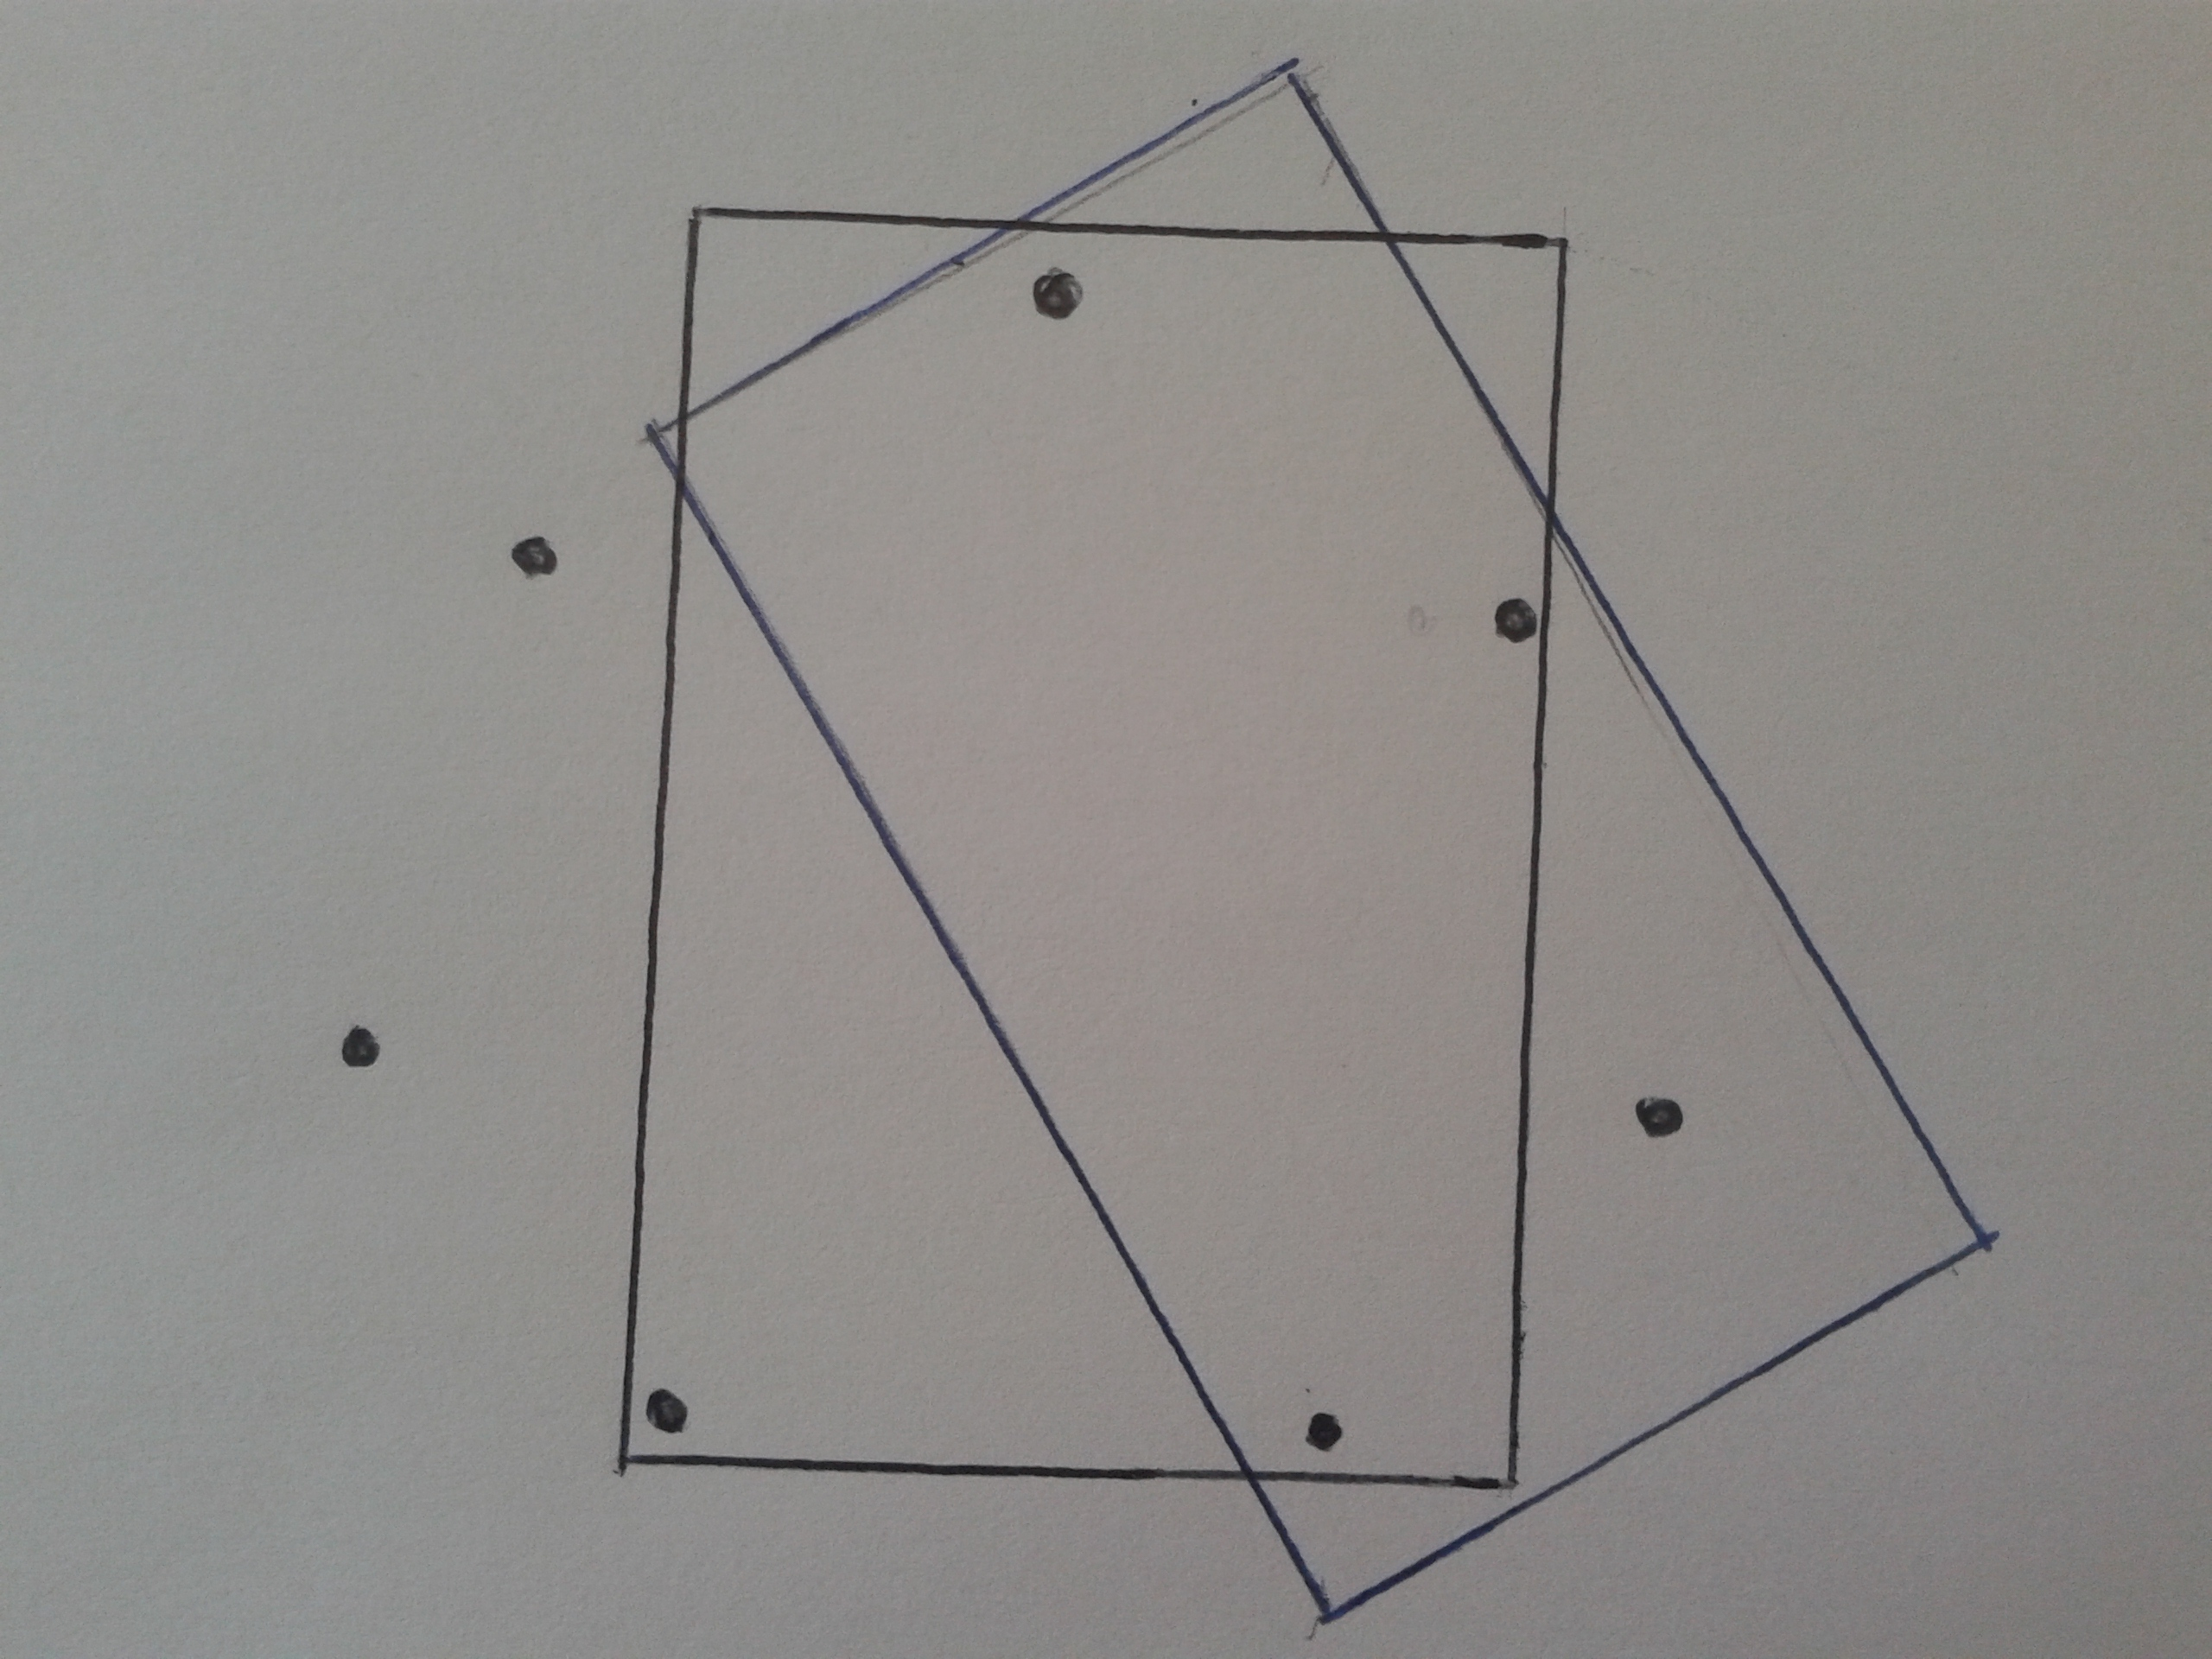
\includegraphics[width=.6\linewidth]{23.jpg}

If you try for 8 points, this construction will fail already with a subset of 3.
We know because of the beginning, that they have to be in a ring organized. If you
have that then the following is a counterexample of a subset. You can try to
draw the points a little bit different, but because of the symmetry you will
always have the same problem for a subset. 

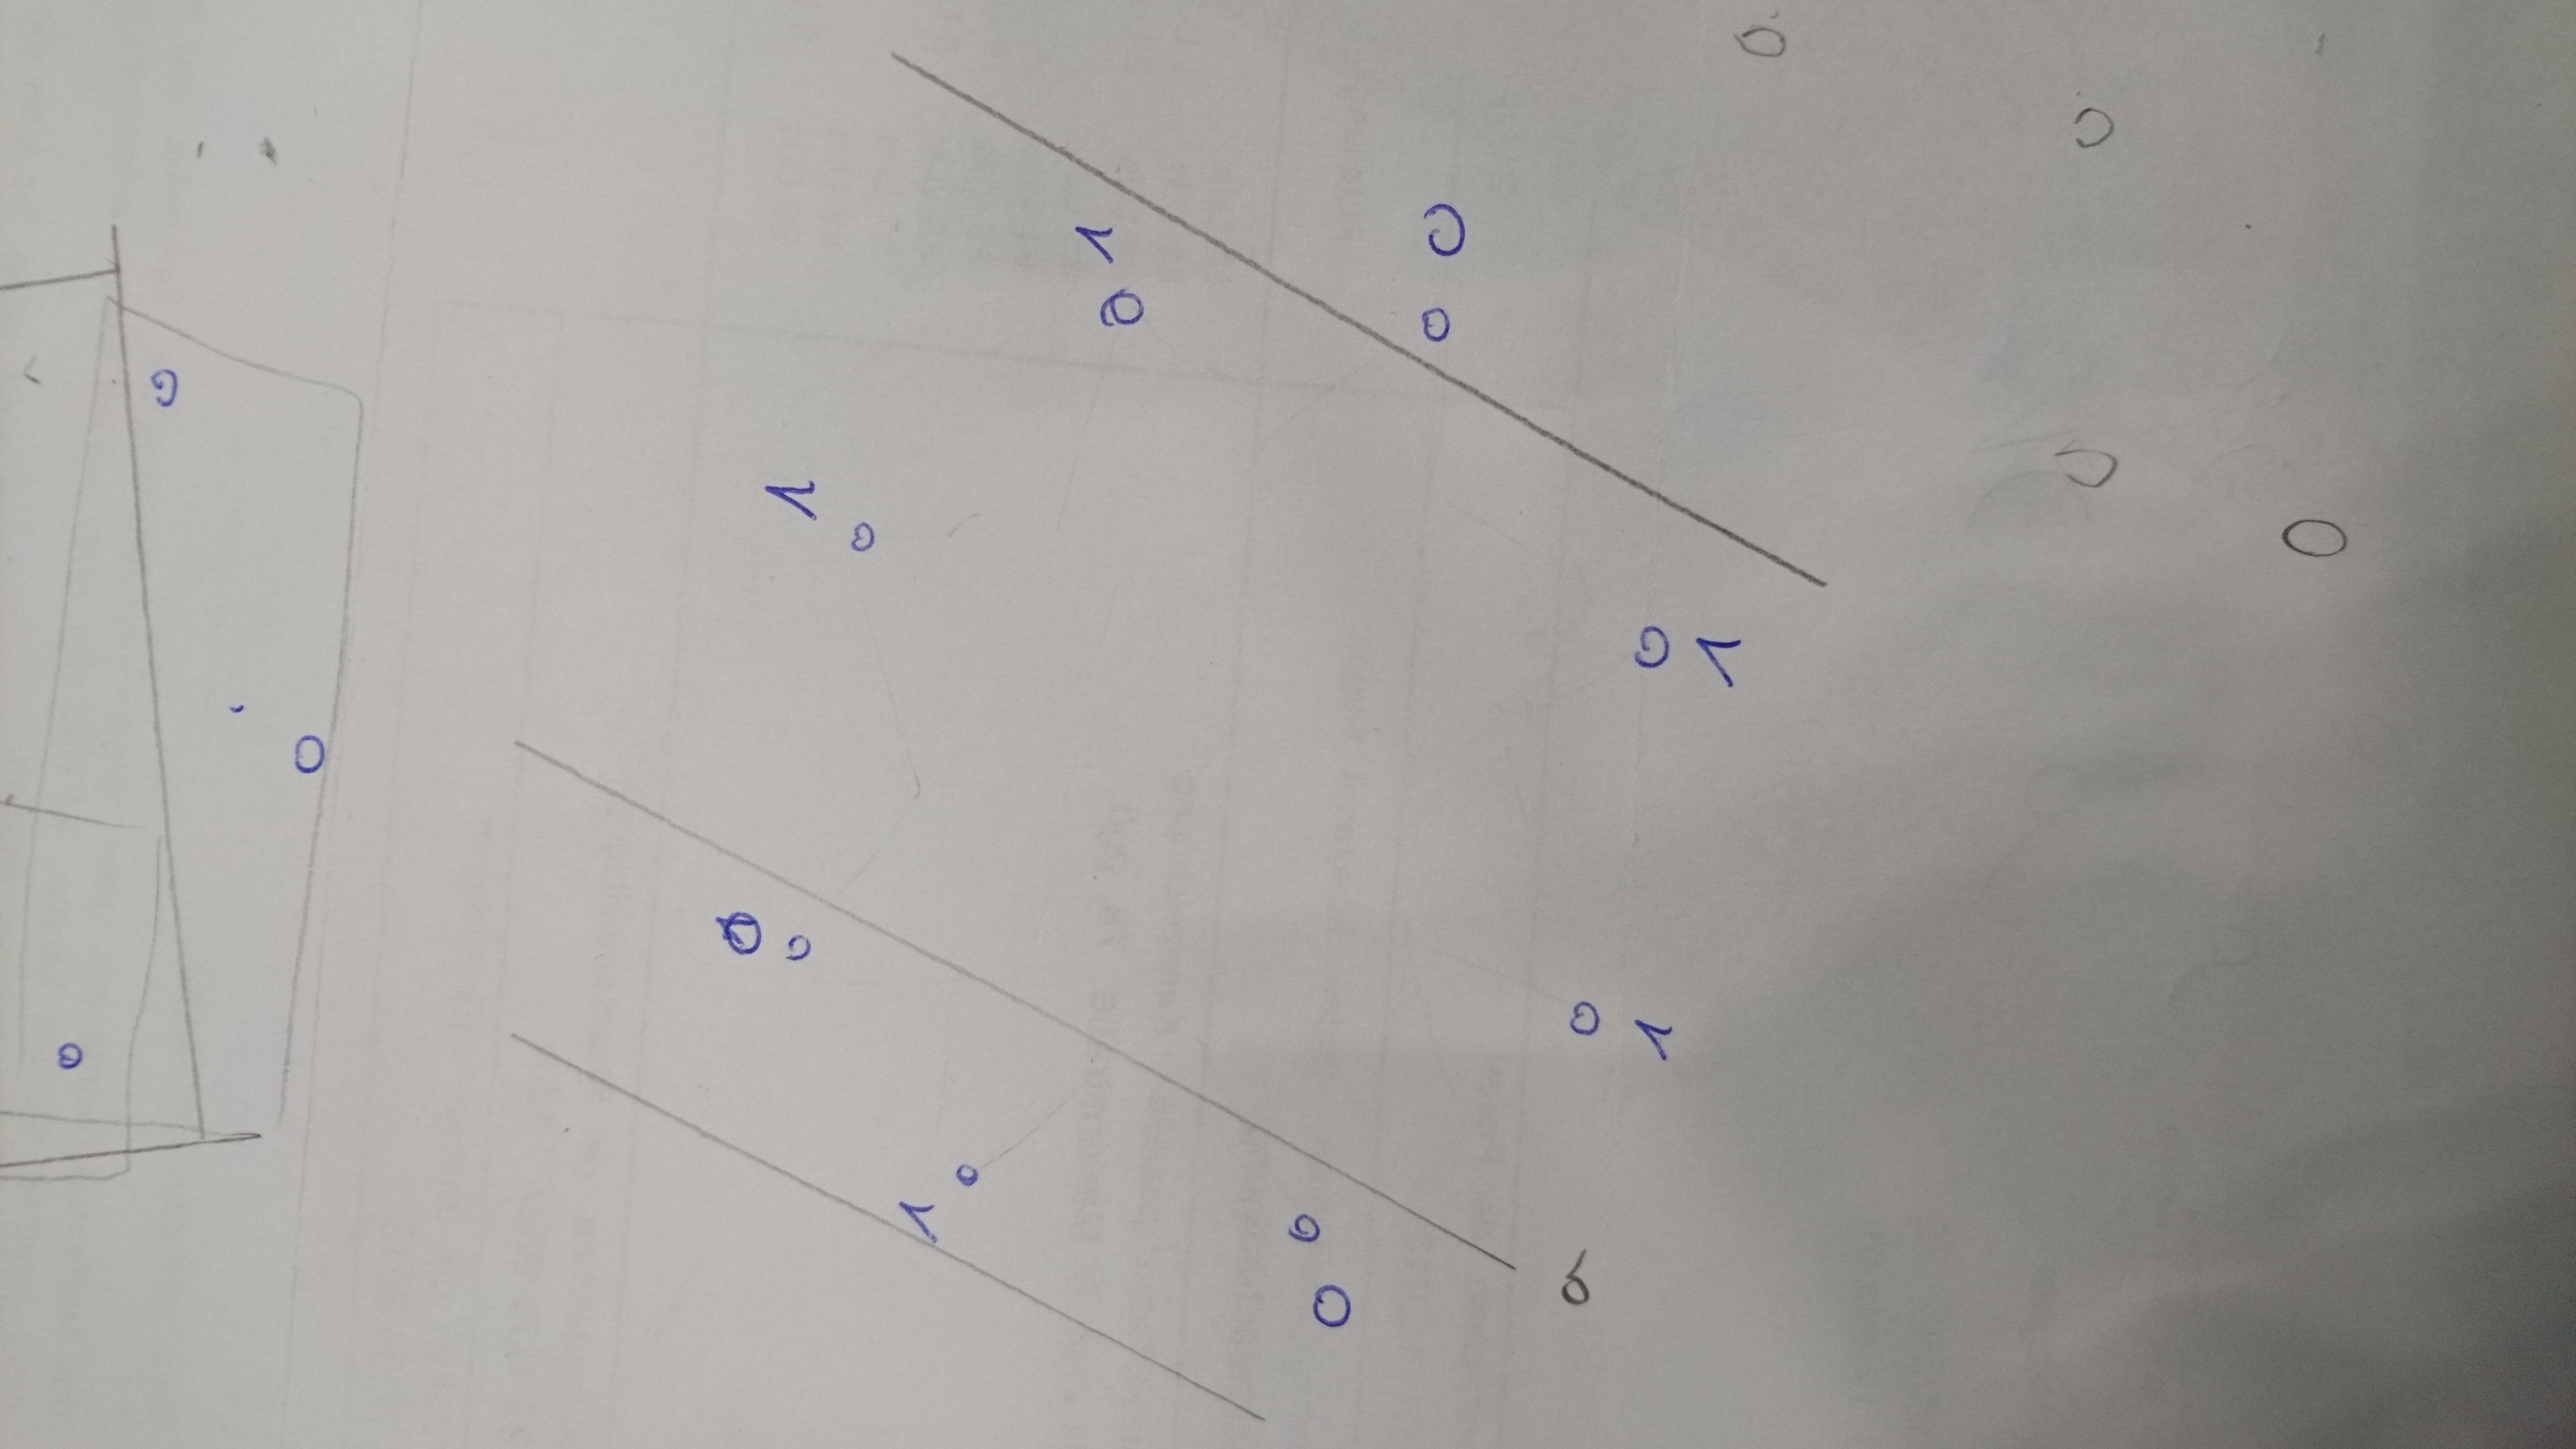
\includegraphics[width=.6\linewidth]{22.jpg}

\end{document}
